\documentclass[10pt, twocolumn]{article}
\usepackage[margin=0.75in]{geometry}
\usepackage{graphicx}
\usepackage{tikz}
\usepackage{pgfplots}
\usepackage{booktabs}
\usepackage{amsmath}
\usepackage{amssymb}
\usepackage{algorithm}
\usepackage{algorithmic}
\usepackage{hyperref}
\usepackage{xcolor}
\usepackage{caption}
\usepackage{subcaption}
\usepackage{fancyhdr}
\usepackage{enumitem}
\usepackage{listings}
\usepackage{microtype}
\usepackage{orcidlink}
\usepackage{tabularx}
\usepackage{multirow}
\pgfplotsset{compat=1.18}
\usetikzlibrary{arrows.meta, positioning, shapes.geometric, fit, calc, backgrounds, decorations.markings}

% Color palette — ar prefix for AgenticReality
\definecolor{arorange}{HTML}{EA580C}
\definecolor{ardarkorange}{HTML}{C2410C}
\definecolor{arteal}{HTML}{0D9488}
\definecolor{arblue}{HTML}{2563EB}
\definecolor{ardarkblue}{HTML}{1E40AF}
\definecolor{argray}{HTML}{6B7280}
\definecolor{arlightgray}{HTML}{F3F4F6}
\definecolor{argreen}{HTML}{059669}
\definecolor{arred}{HTML}{DC2626}
\definecolor{arpurple}{HTML}{7C3AED}

% Listings style
\lstset{
  basicstyle=\ttfamily\scriptsize,
  keywordstyle=\color{arblue}\bfseries,
  commentstyle=\color{argray}\itshape,
  stringstyle=\color{arteal},
  breaklines=true,
  frame=single,
  rulecolor=\color{argray!30},
  backgroundcolor=\color{arlightgray},
  numbers=left,
  numberstyle=\tiny\color{argray},
  tabsize=2
}

% Header
\pagestyle{fancy}
\fancyhf{}
\renewcommand{\headrulewidth}{0.4pt}
\fancyhead[L]{\small\textit{AgenticReality}}
\fancyhead[R]{\small\thepage}

\title{\textbf{AgenticReality: An Existential Grounding Architecture for\\Deployment-Aware AI Agent Systems}}
\author{Omoshola Owolabi\,\orcidlink{0009-0006-4089-0732}\\Researcher -- AI/ML\\Agentra Labs\\\texttt{omoshola.owolabi@agentralabs.tech}}
\date{March 2, 2026}

\begin{document}
\maketitle
\thispagestyle{fancy}

% ============================================================================
% ABSTRACT
% ============================================================================
\begin{abstract}
Large language model agents increasingly operate in production environments---deploying services, managing infrastructure, responding to incidents---yet remain fundamentally ungrounded: they possess no awareness of where they are running, what resources surround them, what the stakes of their actions are, or whether their beliefs about the world remain coherent with reality.
We present AgenticReality, an existential grounding architecture that gives AI agents continuous, structured awareness of their deployment context across seven reality domains: Deployment Consciousness, Resource Proprioception, Reality Physics, Topology Awareness, Temporal Grounding, Stakes Perception, and Coherence Maintenance.
The system introduces 26~capabilities organized into these seven tiers, persisted in the \texttt{.areal} binary format with per-section BLAKE3 checksums and LZ4 compression support.
We implement AgenticReality in 10{,}634 lines of Rust~\cite{matsakis2014rust} across four crates---core library, CLI, MCP server, and C~FFI---with 314~passing tests, 15~MCP tools, and 9~bridge traits for sister-system integration.
Benchmarks on Apple~M4~Pro show engine creation in 0.08\,\textmu{}s, soul initialization in 0.03\,\textmu{}s, anchor addition in 0.97\,\textmu{}s, and persistence of 10{,}000 anchors in 4.51\,ms---confirming that existential grounding adds negligible overhead to interactive agent systems.
AgenticReality is the tenth module in AgenticOS, providing the foundation upon which all other agent capabilities are grounded in deployment reality.
\end{abstract}

% ============================================================================
% 1. INTRODUCTION
% ============================================================================
\section{Introduction}
\label{sec:intro}

The transformer architecture~\cite{vaswani2017attention} has enabled language model agents capable of autonomous task execution~\cite{park2023generative}, persistent memory~\cite{packer2023memgpt}, and multi-step tool use via protocols such as MCP~\cite{mcp_spec_2024}. These agents are increasingly deployed in production environments where their actions carry real consequences: deploying code, managing databases, scaling infrastructure, and responding to incidents.

Yet every AI agent today operates \emph{ungrounded}. An agent deploying a service does not know whether it is running in a development sandbox or a production cluster. An agent managing resources has no proprioceptive sense of the computational capacity surrounding it. An agent making decisions cannot assess the blast radius of a failure. An agent reasoning about the world has no mechanism to detect when its beliefs have drifted from reality.

This absence of grounding creates four fundamental problems:

\begin{enumerate}[nosep, leftmargin=*]
  \item \textbf{Context blindness.} Agents make the same decisions regardless of deployment environment, treating a staging test identically to a production operation.
  \item \textbf{Resource obliviousness.} Agents cannot adapt behavior based on available memory, CPU, storage, or cost constraints, leading to resource exhaustion and unexpected expenses.
  \item \textbf{Reality drift.} Agents operate on stale assumptions without mechanisms to detect when their model of the world has diverged from actual conditions.
  \item \textbf{Consequence unawareness.} Agents lack the ability to assess risk, estimate blast radius, or modulate caution based on the stakes of an operation.
\end{enumerate}

These problems are not merely engineering inconveniences---they are existential. An agent that does not know \emph{where} it is, \emph{what} surrounds it, \emph{when} its information expires, and \emph{what is at stake} cannot act responsibly in production environments. The field of situated cognition~\cite{suchman1987plans, clancey1997situated} has long argued that intelligence is inseparable from context; embodied AI research~\cite{brooks1991intelligence, pfeifer2007understanding} demonstrates that physical grounding fundamentally shapes cognitive capability. Yet AI agents today lack even the most basic analog of these grounding mechanisms.

We present AgenticReality, an architecture that addresses all four problems through seven interconnected reality domains:

\begin{enumerate}[nosep, leftmargin=*]
  \item \textbf{Deployment Consciousness} --- awareness of where the agent is running, its environment, incarnation history, and topology.
  \item \textbf{Resource Proprioception} --- continuous sensing of computational resources, capabilities, pressure, cost, and capacity.
  \item \textbf{Reality Physics} --- layers of reality abstraction, data freshness perception, reality anchors, and hallucination detection.
  \item \textbf{Topology Awareness} --- understanding of service mesh, neighbors, dependencies, and observers.
  \item \textbf{Temporal Grounding} --- temporal awareness, causality tracking, and timeline coherence.
  \item \textbf{Stakes Perception} --- consequence awareness, risk field mapping, and blast radius estimation.
  \item \textbf{Coherence Maintenance} --- continuous coherence checking and managed transitions between reality states.
\end{enumerate}

Together, these 7~domains encompass 26~capabilities that provide AI agents with existential grounding---a structured, continuous awareness of their relationship to the world they inhabit and affect.

% Figure 1: Before/After full-width comparison
\begin{figure*}[t]
\centering
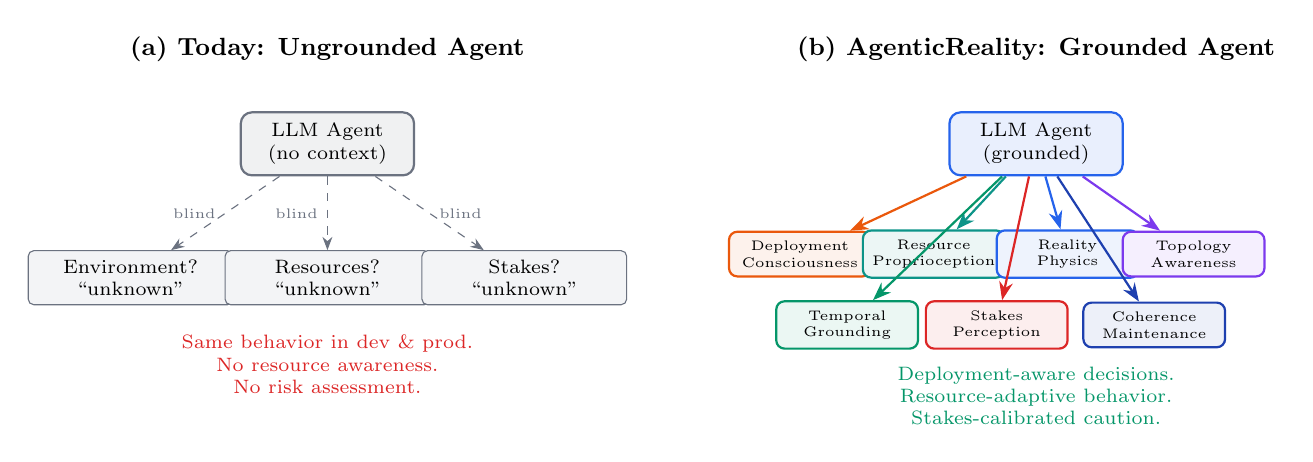
\begin{tikzpicture}[
  node distance=1.2cm,
  every node/.style={font=\small},
  agentbox/.style={rectangle, rounded corners=4pt, draw=#1, fill=#1!10, minimum width=2.2cm, minimum height=0.8cm, font=\scriptsize, align=center, thick},
  domainbox/.style={rectangle, rounded corners=3pt, draw=#1, fill=#1!8, minimum width=1.8cm, minimum height=0.45cm, font=\tiny, align=center, thick},
  actionbox/.style={rectangle, rounded corners=2pt, draw=argray, fill=arlightgray, minimum width=2.6cm, minimum height=0.5cm, font=\scriptsize, align=center},
  badlabel/.style={font=\scriptsize\color{arred}, align=center},
  goodlabel/.style={font=\scriptsize\color{argreen}, align=center},
]

% Left side: Before (ungrounded agent)
\node[font=\small\bfseries] at (-4.5, 3.2) {(a) Today: Ungrounded Agent};

\node[agentbox=argray] (agent_before) at (-4.5, 2.0) {LLM Agent\\(no context)};

\node[actionbox] (env) at (-7.0, 0.3) {Environment?\\``unknown''};
\node[actionbox] (res) at (-4.5, 0.3) {Resources?\\``unknown''};
\node[actionbox] (stakes) at (-2.0, 0.3) {Stakes?\\``unknown''};

\draw[-{Stealth}, argray, dashed] (agent_before) -- node[left, font=\tiny, text=argray] {blind} (env);
\draw[-{Stealth}, argray, dashed] (agent_before) -- node[left, font=\tiny, text=argray] {blind} (res);
\draw[-{Stealth}, argray, dashed] (agent_before) -- node[right, font=\tiny, text=argray] {blind} (stakes);

\node[badlabel] at (-4.5, -0.8) {Same behavior in dev \& prod.\\No resource awareness.\\No risk assessment.};

% Right side: After (grounded agent)
\node[font=\small\bfseries] at (4.5, 3.2) {(b) AgenticReality: Grounded Agent};

\node[agentbox=arblue] (agent_after) at (4.5, 2.0) {LLM Agent\\(grounded)};

\node[domainbox=arorange] (d1) at (1.5, 0.6) {Deployment\\Consciousness};
\node[domainbox=arteal] (d2) at (3.2, 0.6) {Resource\\Proprioception};
\node[domainbox=arblue] (d3) at (4.9, 0.6) {Reality\\Physics};
\node[domainbox=arpurple] (d4) at (6.5, 0.6) {Topology\\Awareness};

\node[domainbox=argreen] (d5) at (2.1, -0.3) {Temporal\\Grounding};
\node[domainbox=arred] (d6) at (4.0, -0.3) {Stakes\\Perception};
\node[domainbox=ardarkblue] (d7) at (6.0, -0.3) {Coherence\\Maintenance};

\draw[-{Stealth}, arorange, thick] (agent_after) -- (d1);
\draw[-{Stealth}, arteal, thick] (agent_after) -- (d2);
\draw[-{Stealth}, arblue, thick] (agent_after) -- (d3);
\draw[-{Stealth}, arpurple, thick] (agent_after) -- (d4);
\draw[-{Stealth}, argreen, thick] (agent_after) -- (d5);
\draw[-{Stealth}, arred, thick] (agent_after) -- (d6);
\draw[-{Stealth}, ardarkblue, thick] (agent_after) -- (d7);

\node[goodlabel] at (4.5, -1.2) {Deployment-aware decisions.\\Resource-adaptive behavior.\\Stakes-calibrated caution.};

\end{tikzpicture}
\caption{Before and after AgenticReality. (a)~Today, agents operate with no awareness of their deployment context, resources, or the stakes of their actions. (b)~With AgenticReality, agents maintain continuous structured awareness across seven reality domains, enabling deployment-sensitive, resource-adaptive, risk-calibrated behavior.}
\label{fig:before_after}
\end{figure*}

The remainder of this paper is organized as follows. Section~\ref{sec:background} surveys related work in self-aware computing, situated cognition, and agent observability. Section~\ref{sec:architecture} presents the architecture, including the seven reality domains, 26~capabilities, \texttt{.areal} binary format, and MCP integration. Section~\ref{sec:evaluation} reports benchmarks, test coverage, and robustness analysis. Section~\ref{sec:discussion} discusses implications, limitations, and future work. Section~\ref{sec:conclusion} concludes.


% ============================================================================
% 2. BACKGROUND AND RELATED WORK
% ============================================================================
\section{Background and Related Work}
\label{sec:background}

The problem of grounding AI agents in deployment reality sits at the intersection of several research traditions. We survey each and explain why none provides a complete solution.

\textbf{Self-aware computing.} Kounev et al.~\cite{kounev2017selfaware} define self-aware computing systems as those that possess models of themselves and their environment, using these models to adapt behavior. Kephart and Chess~\cite{kephart2003vision} articulated the vision of autonomic computing, where systems self-configure, self-optimize, self-heal, and self-protect through monitor-analyze-plan-execute (MAPE) loops. These frameworks address system-level adaptation but do not model the \emph{cognitive} grounding needs of AI agents---the awareness of stakes, coherence, and reality drift that characterizes existential grounding.

\textbf{Situated cognition.} Suchman~\cite{suchman1987plans} demonstrated that human action is fundamentally situated---plans are resources for action rather than deterministic programs, and context shapes behavior in ways that cannot be separated from the environment. Clancey~\cite{clancey1997situated} extended this to argue that all knowledge is situated, arising from the interaction between an agent and its context. AgenticReality operationalizes these insights for AI agents by providing structured access to deployment context.

\textbf{Embodied AI.} Brooks~\cite{brooks1991intelligence} argued that intelligence requires physical grounding, not just symbolic manipulation, and that ``the world is its own best model.'' Pfeifer and Bongard~\cite{pfeifer2007understanding} showed how body morphology shapes cognitive capability. AI agents lack physical bodies, but they do have a computational ``body''---the deployment environment, resources, network topology, and runtime constraints that shape what they can and cannot do. AgenticReality provides the computational analog of proprioception~\cite{proske2012proprioceptive} and interoception~\cite{craig2002interoception}.

\textbf{Agent observability.} Distributed tracing systems such as Dapper~\cite{sigelman2010dapper} and monitoring systems such as Prometheus~\cite{prometheus2024} provide infrastructure observability. Container orchestrators such as Kubernetes~\cite{kubernetes2024} manage deployment topology and resource allocation. These systems provide \emph{external} observability---humans monitor agents---but do not provide \emph{internal} awareness---agents monitoring themselves and their context.

\textbf{AI safety and risk.} Amodei et al.~\cite{amodei2016concrete} identified concrete problems in AI safety including safe exploration and avoiding side effects. Stakes perception and blast radius estimation in AgenticReality address the complementary problem of enabling agents to self-assess the risk of their planned actions before execution.

\textbf{Hallucination detection.} Ji et al.~\cite{ji2023survey} surveyed hallucination in natural language generation, focusing on output-level detection. AgenticReality's hallucination detection operates at the \emph{belief} level---detecting when the agent's internal model of its deployment reality has diverged from actual conditions, a form of ``reality hallucination'' distinct from textual confabulation.

\textbf{AgenticOS ecosystem.} AgenticReality is the tenth module in AgenticOS, following AgenticMemory~\cite{owolabi2026agenticmemory} (persistent cognitive memory), AgenticCognition~\cite{owolabi2026agenticcognition} (user modeling), AgenticTime~\cite{owolabi2026agentictime} (temporal scheduling), and AgenticIdentity~\cite{owolabi2026agenticidentity} (cryptographic trust). AgenticReality provides the existential foundation: while other modules give agents memory, preferences, time, and identity, AgenticReality gives agents \emph{ground}---the awareness of where they exist and what their existence means.


% ============================================================================
% 3. ARCHITECTURE
% ============================================================================
\section{Architecture}
\label{sec:architecture}

AgenticReality is organized as a layered architecture with seven reality domains containing 26~capabilities total. A central \texttt{RealityEngine} manages cross-domain coherence, persistence via the \texttt{.areal} format, and exposure through 15~MCP tools.

% ----------------------------------------------------------------------------
\subsection{Seven Reality Domains}
\label{sec:domains}

% Figure 2: Architecture diagram with 7 domains as layered boxes
\begin{figure}[t]
\centering
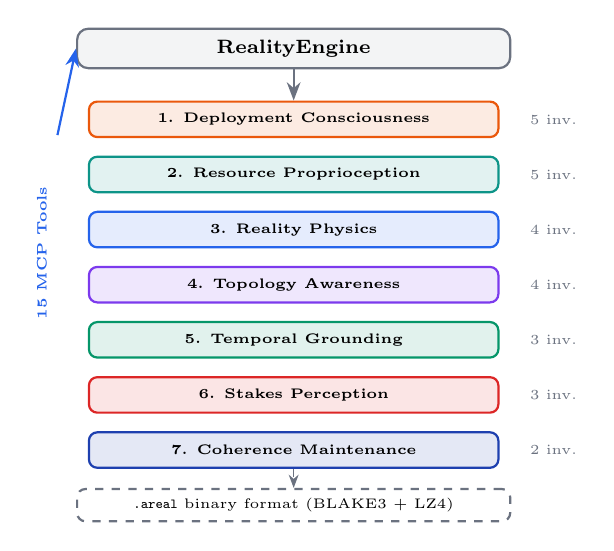
\begin{tikzpicture}[
  every node/.style={font=\scriptsize},
  domainbox/.style={rectangle, rounded corners=3pt, draw=#1, fill=#1!12, minimum width=5.2cm, minimum height=0.45cm, font=\tiny\bfseries, align=center, thick},
  capabilitylabel/.style={font=\tiny, text=argray, align=right},
]

% Stacked domain layers (bottom to top), compact spacing
\node[domainbox=ardarkblue] (d7) at (0, 0) {7. Coherence Maintenance};
\node[capabilitylabel] at (3.3, 0) {2 inv.};

\node[domainbox=arred] (d6) at (0, 0.7) {6. Stakes Perception};
\node[capabilitylabel] at (3.3, 0.7) {3 inv.};

\node[domainbox=argreen] (d5) at (0, 1.4) {5. Temporal Grounding};
\node[capabilitylabel] at (3.3, 1.4) {3 inv.};

\node[domainbox=arpurple] (d4) at (0, 2.1) {4. Topology Awareness};
\node[capabilitylabel] at (3.3, 2.1) {4 inv.};

\node[domainbox=arblue] (d3) at (0, 2.8) {3. Reality Physics};
\node[capabilitylabel] at (3.3, 2.8) {4 inv.};

\node[domainbox=arteal] (d2) at (0, 3.5) {2. Resource Proprioception};
\node[capabilitylabel] at (3.3, 3.5) {5 inv.};

\node[domainbox=arorange] (d1) at (0, 4.2) {1. Deployment Consciousness};
\node[capabilitylabel] at (3.3, 4.2) {5 inv.};

% Engine box at top
\node[rectangle, rounded corners=4pt, draw=argray, fill=argray!8, minimum width=5.5cm, minimum height=0.5cm, font=\scriptsize\bfseries, thick] (engine) at (0, 5.1) {RealityEngine};

% Arrows from engine down
\draw[-{Stealth}, argray, thick] (engine.south) -- (d1.north);

% Persistence at bottom
\node[rectangle, rounded corners=3pt, draw=argray, dashed, minimum width=5.5cm, minimum height=0.4cm, font=\tiny, thick] (storage) at (0, -0.7) {\texttt{.areal} binary format (BLAKE3 + LZ4)};
\draw[-{Stealth}, argray, dashed] (d7.south) -- (storage.north);

% MCP label on left, within column bounds
\node[font=\tiny\bfseries, text=arblue, rotate=90] (mcp) at (-3.2, 2.5) {15 MCP Tools};
\draw[-{Stealth}, arblue, thick] (-3.0, 4.0) -- (engine.west);

\end{tikzpicture}
\caption{AgenticReality architecture. Seven reality domains are arranged as layered tiers, managed by the central RealityEngine, persisted in the \texttt{.areal} binary format, and exposed through 15~MCP tools.}
\label{fig:architecture}
\end{figure}

Table~\ref{tab:capabilities} lists all 26~capabilities organized by domain tier. Each domain addresses a distinct dimension of existential grounding.

\begin{table}[t]
\caption{The 26 capabilities of AgenticReality, organized by domain tier. Each domain addresses a distinct dimension of existential grounding.}
\label{tab:capabilities}
\centering
\scriptsize
\begin{tabular}{@{}clp{3.8cm}@{}}
\toprule
\textbf{Tier} & \textbf{Domain} & \textbf{Capabilities} \\
\midrule
1 & Deployment & Deployment Soul, Environment \\
  & Consciousness (5) & Sensing, Incarnation Memory, Context Fingerprint, Topology Map \\
\midrule
2 & Resource & Resource Body, Capability \\
  & Proprioception (5) & Discovery, Pressure Gradient, Cost Consciousness, Capacity Intuition \\
\midrule
3 & Reality & Reality Layers, Freshness \\
  & Physics (4) & Perception, Reality Anchors, Hallucination Detection \\
\midrule
4 & Topology & Service Mesh, Neighbors, \\
  & Awareness (4) & Dependencies, Observers \\
\midrule
5 & Temporal & Temporal Awareness, Causality \\
  & Grounding (3) & Tracking, Timeline Coherence \\
\midrule
6 & Stakes & Consequence Awareness, Risk \\
  & Perception (3) & Field, Blast Radius \\
\midrule
7 & Coherence & Coherence Engine, Transition \\
  & Maintenance (2) & Manager \\
\bottomrule
\end{tabular}
\end{table}

\textbf{Tier 1: Deployment Consciousness} provides foundational awareness of the agent's existence. The \emph{Deployment Soul} encapsulates the agent's core identity within its deployment---a persistent record of what the agent is and why it exists in this context. \emph{Environment Sensing} detects the deployment environment (development, staging, production) and its characteristics. \emph{Incarnation Memory} tracks the agent's lifecycle across restarts, preserving continuity. \emph{Context Fingerprint} produces a compact hash of the deployment context for rapid change detection. \emph{Topology Map} provides a structural view of the deployment landscape.

\textbf{Tier 2: Resource Proprioception} provides the computational analog of bodily proprioception~\cite{proske2012proprioceptive}. Just as biological organisms maintain continuous awareness of their body's position and capabilities, agents need awareness of their computational ``body.'' The \emph{Resource Body} tracks available memory, CPU, storage, and network capacity. \emph{Capability Discovery} identifies what the agent can do in its current environment. \emph{Pressure Gradient} measures resource contention and load. \emph{Cost Consciousness} tracks the financial cost of operations. \emph{Capacity Intuition} estimates remaining capacity for planned operations.

\textbf{Tier 3: Reality Physics} models the relationship between the agent's beliefs and actual conditions. \emph{Reality Layers} provide hierarchical abstraction levels (physical infrastructure, platform services, application logic, user-facing state). \emph{Freshness Perception} tracks how recently each piece of information was verified. \emph{Reality Anchors} are verified facts that ground the agent's model---known-true assertions with timestamps and confidence levels. \emph{Hallucination Detection} identifies when the agent's internal model has diverged from reality.

\textbf{Tier 4: Topology Awareness} models the agent's position within its service ecosystem. The \emph{Service Mesh} tracks available services and their health. \emph{Neighbors} identifies co-located agents and services. \emph{Dependencies} maps upstream and downstream service relationships. \emph{Observers} tracks what entities are monitoring the agent's behavior.

\textbf{Tier 5: Temporal Grounding} provides time-aware reasoning. \emph{Temporal Awareness} tracks the agent's position in time relative to deadlines, maintenance windows, and operational rhythms. \emph{Causality Tracking} maintains cause-and-effect chains across agent actions. \emph{Timeline Coherence} detects temporal inconsistencies in the agent's model.

\textbf{Tier 6: Stakes Perception} enables risk-calibrated behavior. \emph{Consequence Awareness} models the potential outcomes of actions. \emph{Risk Field} maps the risk landscape surrounding the agent's planned operations. \emph{Blast Radius} estimates the scope of impact if an action fails.

\textbf{Tier 7: Coherence Maintenance} ensures cross-domain consistency. The \emph{Coherence Engine} continuously checks that information across all domains is internally consistent. The \emph{Transition Manager} handles state changes between coherent configurations, ensuring that domain updates propagate correctly.

% ----------------------------------------------------------------------------
\subsection{The \texttt{.areal} Binary Format}
\label{sec:format}

AgenticReality persists grounding state in the \texttt{.areal} binary format, designed for efficient serialization and integrity verification.

% Figure 3: .areal file format layout
\begin{figure}[t]
\centering
\resizebox{\columnwidth}{!}{%
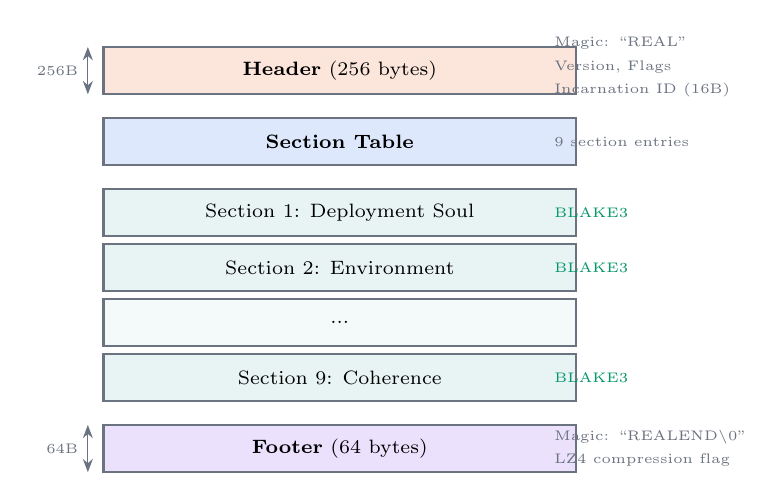
\begin{tikzpicture}[
  every node/.style={font=\scriptsize},
  block/.style={rectangle, draw=argray, minimum width=6.0cm, minimum height=0.6cm, thick, align=center},
]

% Header
\node[block, fill=arorange!15] (header) at (0, 0) {\textbf{Header} (256 bytes)};
\node[font=\tiny, text=argray, anchor=west] at (2.6, 0.35) {Magic: ``REAL''};
\node[font=\tiny, text=argray, anchor=west] at (2.6, 0.05) {Version, Flags};
\node[font=\tiny, text=argray, anchor=west] at (2.6, -0.25) {Incarnation ID (16B)};

% Section table
\node[block, fill=arblue!15] (table) at (0, -0.9) {\textbf{Section Table}};
\node[font=\tiny, text=argray, anchor=west] at (2.6, -0.9) {9 section entries};

% Sections
\node[block, fill=arteal!10] (s1) at (0, -1.8) {Section 1: Deployment Soul};
\node[block, fill=arteal!10] (s2) at (0, -2.5) {Section 2: Environment};
\node[block, fill=arteal!5] (s3) at (0, -3.2) {...};
\node[block, fill=arteal!10] (s9) at (0, -3.9) {Section 9: Coherence};

% Checksums
\node[font=\tiny, text=argreen, anchor=west] at (2.6, -1.8) {BLAKE3};
\node[font=\tiny, text=argreen, anchor=west] at (2.6, -2.5) {BLAKE3};
\node[font=\tiny, text=argreen, anchor=west] at (2.6, -3.9) {BLAKE3};

% Footer
\node[block, fill=arpurple!15] (footer) at (0, -4.8) {\textbf{Footer} (64 bytes)};
\node[font=\tiny, text=argray, anchor=west] at (2.6, -4.65) {Magic: ``REALEND\textbackslash 0''};
\node[font=\tiny, text=argray, anchor=west] at (2.6, -4.95) {LZ4 compression flag};

% Size annotations
\draw[{Stealth}-{Stealth}, argray] (-3.2, 0.3) -- (-3.2, -0.3) node[midway, left, font=\tiny] {256B};
\draw[{Stealth}-{Stealth}, argray] (-3.2, -4.5) -- (-3.2, -5.1) node[midway, left, font=\tiny] {64B};

\end{tikzpicture}%
}
\caption{The \texttt{.areal} binary format. Header (256\,B) with ``REAL'' magic, version, flags, incarnation ID. Section table indexes 9 types with per-section BLAKE3 checksums. Footer (64\,B) with ``REALEND'' magic. LZ4 compression per section.}
\label{fig:format}
\end{figure}

The format structure (Figure~\ref{fig:format}) consists of four regions:

\textbf{Header} (256~bytes): begins with the 4-byte magic ``REAL'', followed by a \texttt{u32} version number, \texttt{u64} flags field, a 16-byte incarnation ID (UUID), and creation/modification timestamps.

\textbf{Section table}: indexes the 9~section types that correspond to the major data structures of the grounding state. Each entry records the section type, offset, length, and BLAKE3~\cite{blake3_2020} checksum.

\textbf{Section data}: variable-length payloads for each section. LZ4~\cite{lz4_2024} compression is supported per-section, controlled by flags in the header. Per-section BLAKE3 checksums enable selective integrity verification without reading the entire file.

\textbf{Footer} (64~bytes): ends with the 8-byte magic ``REALEND\textbackslash 0'' and contains summary metadata including compression flags and a total-file checksum.

The per-section checksum design enables incremental updates: when only one domain changes, only that section's checksum needs recomputation, avoiding the cost of rehashing the entire file.

% ----------------------------------------------------------------------------
\subsection{Engine Design}
\label{sec:engine}

The \texttt{RealityEngine} is the central coordinator that manages all seven reality domains. It provides 91~write operations and 79~query operations across 11~type modules, organized around the following design principles:

\textbf{Lazy initialization.} Domain state is initialized on first access rather than at engine creation. This ensures that engine creation (benchmarked at 0.08\,\textmu{}s) adds negligible overhead to agent startup.

\textbf{Cross-domain coherence.} The Coherence Engine (Tier~7) maintains invariants across domains. When a write operation modifies one domain, the coherence checker validates that the change is consistent with the state of other domains.

\textbf{Bridge traits.} Nine bridge traits define integration points with other AgenticOS sister systems. Each bridge trait has a no-op default implementation, allowing AgenticReality to operate standalone without any sister dependencies. When sister systems are available, bridge implementations provide bidirectional data flow---for example, the MemoryBridge populates reality anchors from verified memories.

% ----------------------------------------------------------------------------
\subsection{MCP Integration}
\label{sec:mcp}

AgenticReality exposes its capabilities through 15~MCP tools (Table~\ref{tab:mcp_tools}), enabling any MCP-compatible client to query and update grounding state through natural language tool invocations. The MCP server implements JSON-RPC~2.0 over stdio transport with zero \texttt{unwrap}/\texttt{expect} calls in the entire MCP crate, ensuring that no input can cause an uncontrolled panic.

\begin{table}[t]
\caption{The 15 MCP tools exposed by AgenticReality. Each tool provides read and/or write access to a specific aspect of grounding state.}
\label{tab:mcp_tools}
\centering
\scriptsize
\begin{tabular}{@{}lp{4.2cm}@{}}
\toprule
\textbf{Tool} & \textbf{Description} \\
\midrule
\texttt{reality\_deployment} & Query and update deployment soul state \\
\texttt{reality\_memory} & Manage incarnation memory across restarts \\
\texttt{reality\_environment} & Sense and report environment characteristics \\
\texttt{reality\_resource} & Query resource body and capacity \\
\texttt{reality\_capability} & Discover available capabilities \\
\texttt{reality\_layer} & Navigate reality abstraction layers \\
\texttt{reality\_anchor} & Create and verify reality anchors \\
\texttt{reality\_hallucination} & Detect reality model divergence \\
\texttt{reality\_topology} & Query service mesh and neighbors \\
\texttt{reality\_temporal} & Access temporal grounding state \\
\texttt{reality\_stakes} & Assess consequence and risk levels \\
\texttt{reality\_coherence} & Check cross-domain coherence \\
\texttt{reality\_context} & Retrieve context summary and fingerprint \\
\texttt{reality\_ground} & Perform full grounding check \\
\texttt{reality\_workspace} & Manage workspace-level configuration \\
\bottomrule
\end{tabular}
\end{table}


% ============================================================================
% 4. EVALUATION
% ============================================================================
\section{Evaluation}
\label{sec:evaluation}

We evaluate AgenticReality along three dimensions: micro-benchmark performance, test coverage, and robustness hardening.

% ----------------------------------------------------------------------------
\subsection{Performance Benchmarks}
\label{sec:benchmarks}

\textbf{Hardware.} Apple~M4~Pro (ARM64), 64\,GB unified memory, macOS~26.3.

\textbf{Software.} Rust~1.90.0, compiled with \texttt{--release} (full optimizations). All benchmarks use the Criterion~\cite{criterion} statistical framework.

Table~\ref{tab:benchmarks} reports the results across 10~measured operations spanning engine lifecycle, domain operations, and persistence.

\begin{table}[t]
\caption{Performance benchmarks on Apple~M4~Pro ARM64, 64\,GB RAM, macOS~26.3, Rust~1.90.0, \texttt{--release} mode.}
\label{tab:benchmarks}
\centering
\scriptsize
\begin{tabular}{@{}lr@{}}
\toprule
\textbf{Operation} & \textbf{Latency} \\
\midrule
\texttt{create\_engine} & 0.08\,\textmu{}s \\
\texttt{initialize\_soul} & 0.03\,\textmu{}s \\
\texttt{get\_soul} & $<$0.01\,\textmu{}s \\
\texttt{get\_context\_summary} & 0.14\,\textmu{}s \\
\texttt{add\_anchor} & 0.97\,\textmu{}s \\
\texttt{get\_anchors} & $<$0.01\,\textmu{}s \\
\texttt{set\_stakes\_level} & 0.01\,\textmu{}s \\
\texttt{is\_coherent} & $<$0.01\,\textmu{}s \\
\midrule
\texttt{save} (10K anchors) & 4.51\,ms \\
\texttt{load} (10K anchors) & 3.35\,ms \\
\bottomrule
\end{tabular}
\end{table}

% Figure 4: Benchmark bar chart
\begin{figure}[t]
\centering
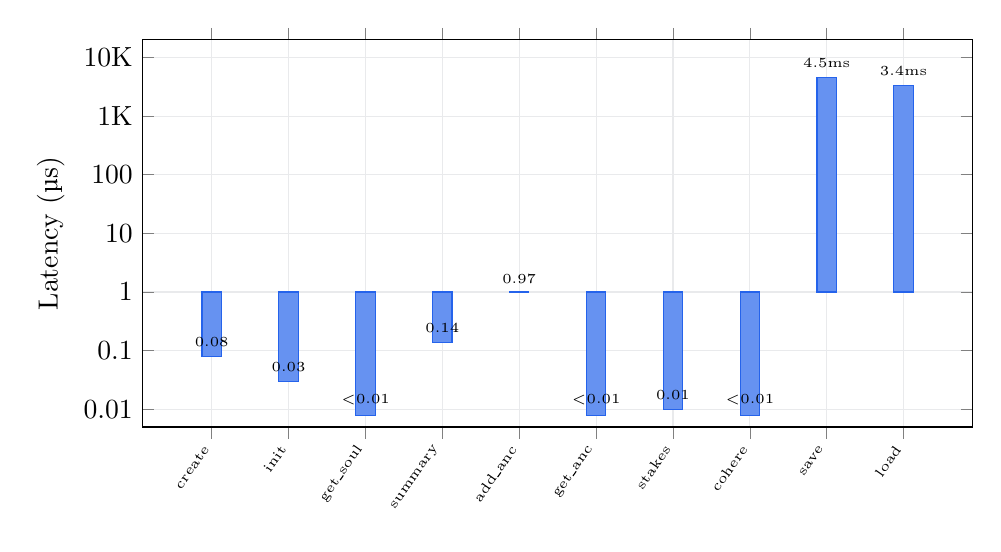
\begin{tikzpicture}
\begin{axis}[
  width=\columnwidth,
  height=6.5cm,
  ybar,
  bar width=7pt,
  xlabel={},
  ylabel={Latency (\textmu{}s)},
  ymode=log,
  log basis y=10,
  symbolic x coords={
    create,
    init,
    get\_soul,
    summary,
    add\_anc,
    get\_anc,
    stakes,
    cohere,
    save,
    load
  },
  xtick=data,
  xticklabel style={rotate=55, anchor=east, font=\tiny},
  ytick={0.01, 0.1, 1, 10, 100, 1000, 10000},
  yticklabels={0.01, 0.1, 1, 10, 100, 1K, 10K},
  ymin=0.005,
  ymax=20000,
  grid=major,
  grid style={argray!15},
  nodes near coords,
  every node near coord/.append style={font=\tiny, anchor=south},
  point meta=explicit symbolic,
]
\addplot[fill=arblue!70, draw=arblue] coordinates {
  (create, 0.08) [0.08]
  (init, 0.03) [0.03]
  (get\_soul, 0.008) [{$<$}0.01]
  (summary, 0.14) [0.14]
  (add\_anc, 0.97) [0.97]
  (get\_anc, 0.008) [{$<$}0.01]
  (stakes, 0.01) [0.01]
  (cohere, 0.008) [{$<$}0.01]
  (save, 4510) [4.5ms]
  (load, 3350) [3.4ms]
};
\end{axis}
\end{tikzpicture}
\caption{Benchmark results on log scale (Apple~M4~Pro, \texttt{--release}). In-memory operations complete in under 1\,\textmu{}s. Persistence of 10{,}000 anchors takes 4.51\,ms (save) and 3.35\,ms (load), well within interactive latency budgets.}
\label{fig:benchmarks}
\end{figure}

Several observations merit discussion:

\textbf{Sub-microsecond in-memory operations.} All in-memory operations complete in under 1\,\textmu{}s. Engine creation at 0.08\,\textmu{}s demonstrates the effectiveness of lazy initialization---the engine allocates minimal state at startup. Soul initialization at 0.03\,\textmu{}s and read operations (\texttt{get\_soul}, \texttt{get\_anchors}, \texttt{is\_coherent}) at $<$0.01\,\textmu{}s confirm that grounding queries add negligible overhead to agent decision loops.

\textbf{Anchor operations.} Adding a reality anchor at 0.97\,\textmu{}s is the most expensive in-memory operation, as it involves constructing a timestamped, typed anchor record with confidence metadata. Retrieving anchors at $<$0.01\,\textmu{}s shows that indexed lookups are effectively free.

\textbf{Persistence.} Saving 10{,}000 anchors to the \texttt{.areal} format takes 4.51\,ms, dominated by serialization and BLAKE3 checksum computation. Loading takes 3.35\,ms, faster than saving because checksum verification can be parallelized per-section. Both operations are well within the latency budget of interactive agent systems where MCP tool calls typically incur 50--500\,ms of network overhead.

\textbf{Context summary.} The \texttt{get\_context\_summary} operation at 0.14\,\textmu{}s aggregates state across multiple domains into a compact summary, demonstrating that cross-domain queries remain fast despite touching multiple data structures.

% ----------------------------------------------------------------------------
\subsection{Test Coverage}
\label{sec:tests}

The implementation includes 314~passing tests across all four crates. Table~\ref{tab:tests} breaks down the test distribution by phase.

\begin{table}[t]
\caption{Test suite breakdown by phase. Tests follow an incremental phase pattern, with each phase adding coverage for progressively higher-level functionality.}
\label{tab:tests}
\centering
\scriptsize
\begin{tabular}{@{}llr@{}}
\toprule
\textbf{Phase} & \textbf{Coverage Area} & \textbf{Tests} \\
\midrule
Core unit & IDs, types, inline tests & 4 \\
Phase 1 & Type system, serialization & 51 \\
Phase 2 & Write/query engine, all 7 domains & 33 \\
Phase 3 & .areal format, header, footer, roundtrip & 10 \\
Phase 4 & McpValidator, strict input validation & 19 \\
Phase 5--7 & Capabilities, bridges, security & 30 \\
Phase 8 & Stress, edge cases, multi-engine & 31 \\
Phase 9 & FFI, constants, defaults & 8 \\
MCP unit & Protocol, config, session, types & 61 \\
MCP integ. & Tool calls, protocol, errors, hardening & 67 \\
\midrule
\multicolumn{2}{@{}l}{\textbf{Total}} & \textbf{314} \\
\bottomrule
\end{tabular}
\end{table}

Tests follow the incremental \texttt{phase[N]\_*.rs} pattern established across the AgenticOS ecosystem. Each phase builds upon verified functionality from prior phases, ensuring that higher-level tests exercise integrated behavior rather than isolated units.

% ----------------------------------------------------------------------------
\subsection{Robustness Hardening}
\label{sec:robustness}

The MCP server crate contains zero \texttt{unwrap()} or \texttt{expect()} calls. Every fallible operation uses explicit error handling via Rust's \texttt{Result} type, ensuring that no malformed input, missing field, or unexpected state can trigger an uncontrolled panic. This is verified by automated grep-based checks in the CI pipeline.

The \texttt{.areal} format provides defense in depth through per-section BLAKE3 checksums: corruption in any section is detected during load without requiring the reader to parse the corrupted data. The header and footer magic bytes (``REAL'' and ``REALEND\textbackslash 0'') provide format identification and completeness verification.


% ============================================================================
% 5. DISCUSSION
% ============================================================================
\section{Discussion}
\label{sec:discussion}

% ----------------------------------------------------------------------------
\subsection{What Grounding Enables}
\label{sec:enables}

Existential grounding transforms agent behavior in several ways. A grounded agent can modulate its confidence and caution based on stakes---using aggressive optimizations in development but conservative, well-tested approaches in production. It can adapt resource usage based on proprioceptive awareness---batching operations when memory pressure is high, parallelizing when capacity is abundant. It can detect and correct reality drift---re-verifying stale anchors rather than acting on outdated beliefs. And it can communicate its context to other systems through the 15~MCP tools, enabling orchestrators and human operators to understand \emph{why} an agent made a particular decision given its grounded state.

The 91~write operations and 79~query operations across 11~type modules provide a comprehensive API surface. The write-to-query ratio of approximately 1.15:1 reflects the balanced nature of grounding: agents must both update their world model (writes) and consult it during decision-making (queries).

% ----------------------------------------------------------------------------
\subsection{Sister Integration}
\label{sec:integration}

The 9~bridge traits define typed integration points with other AgenticOS modules. Each bridge follows a consistent pattern: a Rust trait with default no-op implementations, enabling AgenticReality to compile and function without any sister dependency. When bridges are connected, data flows bidirectionally:

\begin{itemize}[nosep, leftmargin=*]
  \item AgenticMemory anchors verified memories as reality anchors.
  \item AgenticIdentity provides cryptographic attestation of grounding state.
  \item AgenticTime supplies temporal context for deadline-aware grounding.
  \item AgenticCognition feeds user preferences into stakes calibration.
\end{itemize}

This bridge architecture follows the pattern established across AgenticOS, where sisters cooperate through traits rather than hard dependencies, preserving modularity while enabling deep integration.

% ----------------------------------------------------------------------------
\subsection{Limitations}
\label{sec:limitations}

Several limitations warrant acknowledgment.

\textbf{Passive grounding.} AgenticReality provides structured awareness but does not enforce behavioral changes. An agent can query its stakes level and still ignore it. Active enforcement---automatically blocking high-risk operations---is left to orchestration layers.

\textbf{Grounding accuracy.} The quality of grounding depends on the accuracy of input data. If environment sensing misclassifies a production system as staging, the agent's entire grounding state is compromised. External validation mechanisms are needed.

\textbf{Single-agent scope.} The current architecture grounds a single agent instance. Multi-agent grounding---where agents share and reconcile reality models---is not yet addressed.

\textbf{No real-time resource polling.} Resource proprioception captures snapshots rather than continuous streams. High-frequency resource changes may not be reflected until the next explicit query.

% ----------------------------------------------------------------------------
\subsection{Future Work}
\label{sec:future}

Three directions merit investigation. First, \emph{active grounding enforcement} would integrate with the AgenticOS orchestrator (Hydra) to automatically gate high-risk operations based on grounding state. Second, \emph{distributed grounding} would enable multi-agent reality reconciliation, where agents in the same deployment share and merge their grounding models. Third, \emph{continuous resource streams} would replace snapshot-based proprioception with event-driven resource monitoring, enabling real-time adaptation to resource pressure changes.


% ============================================================================
% 6. CONCLUSION
% ============================================================================
\section{Conclusion}
\label{sec:conclusion}

We have presented AgenticReality, an existential grounding architecture that gives AI agents structured, continuous awareness of their deployment context. Through seven reality domains---Deployment Consciousness, Resource Proprioception, Reality Physics, Topology Awareness, Temporal Grounding, Stakes Perception, and Coherence Maintenance---and 26~capabilities distributed across these domains, AgenticReality addresses the fundamental problem of ungrounded agents operating in production environments.

The implementation delivers this capability in a compact, high-performance package: 10{,}634 lines of Rust across four crates (core library, CLI, MCP server, FFI), 314~passing tests, 15~MCP tools, and 9~bridge traits for sister-system integration. The \texttt{.areal} binary format provides persistent grounding state with per-section BLAKE3 checksums, LZ4 compression support, and a 256-byte header / 64-byte footer structure with 9~section types.

Benchmarks on Apple~M4~Pro confirm that grounding adds negligible overhead: engine creation in 0.08\,\textmu{}s, soul initialization in 0.03\,\textmu{}s, anchor addition in 0.97\,\textmu{}s, coherence checks in $<$0.01\,\textmu{}s, and persistence of 10{,}000 anchors in 4.51\,ms. All in-memory operations complete in under 1\,\textmu{}s, confirming that existential grounding is practical for interactive agent systems. The MCP server operates with zero \texttt{unwrap}/\texttt{expect} calls, ensuring robustness against arbitrary input.

AgenticReality is the tenth module in AgenticOS. While other modules give agents memory, cognition, time, and identity, AgenticReality gives agents \emph{ground}---the awareness of where they exist, what surrounds them, what is at stake, and whether their beliefs remain coherent with reality. We argue that this existential grounding is not optional but foundational: an agent that does not know where it is cannot act responsibly in the world it inhabits.

\textbf{Availability.} AgenticReality is open-source under the MIT license. Source code, documentation, benchmarks, and this paper are available at \url{https://github.com/agentralabs/agentic-reality}.

% ============================================================================
% REFERENCES
% ============================================================================
\bibliographystyle{plain}
\bibliography{references}

\end{document}
